\begin{enumerate}
    \item (25\%) Dado el siguiente diagrama de Venn, encuentre $(A^c\cap B)-(B\cap C)$
    \begin{figure}[h]
        \centering
        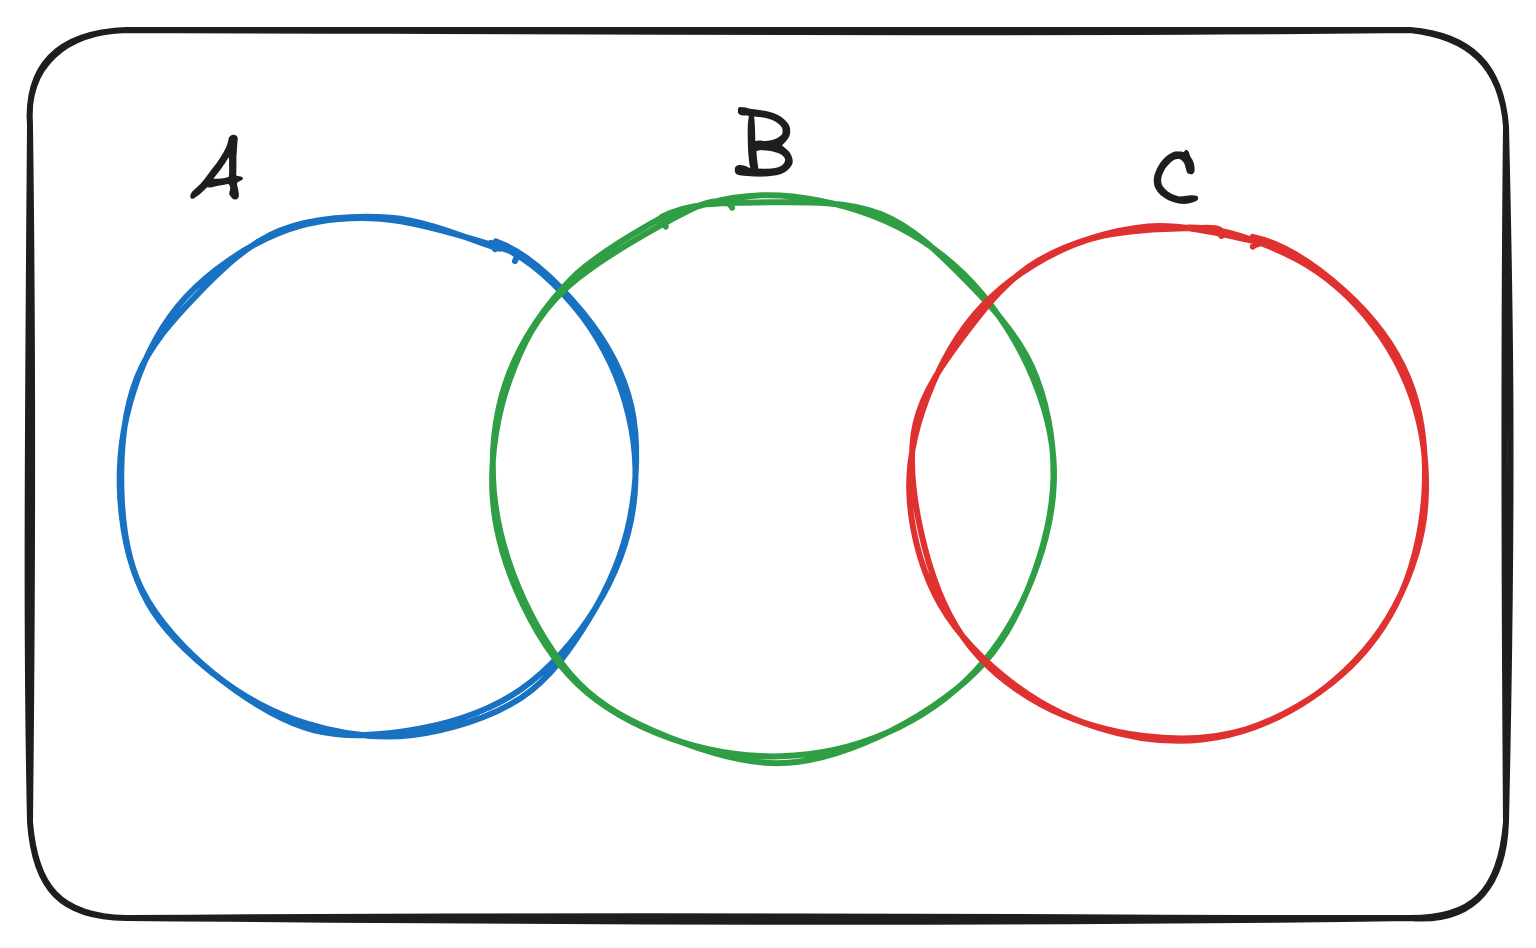
\includegraphics[width=0.3\textwidth]{../Imagenes/IMG1/venn.png}
        \caption{}
        \label{fig:enter-label}
    \end{figure}
    \item (25\%) Realize las siguientes operaciones con los conjuntos $A$, $B$ y $C$.\[A=\{2n + 1 | n \in \mathbb{Z}\}\]\[B=\{x | -2 \leq x < 5\}\]\[C=\{-\pi, -e, \sqrt{2}, 1, 0, -1, \sqrt{3}, \sqrt{49}\}\]
    \begin{multicols}{2}
        \begin{enumerate}
        \item $A\cup B \cup C$.
        \item $(\mathbb{Q}\cap A)\cap B$.
        %\item $((A\cup B)\cap C)\cap \mathbb{R}$.
        %\item $((A-B)\cup (C-A))\cap (B-C)$.
        \item $((C-B)\cup A)-\mathbb{Z}$.
    \end{enumerate}
    \end{multicols}
    %\item (25\%) ¿Cuántos números de tres dígitos $abc$ son tales que $a+3b+c$ es múltiplo de 3?
    \item (25\%) Una cerradura de combinación está numerada del 0 al 30. Una combinación consta de tres números tal que dos números consecutivos deben ser diferentes, pero el primero y el tercero pueden ser iguales. ¿Cuántas combinaciones diferentes son posibles?\\
    \textbf{Ejemplo:} Una combinación válida es 30 29 30.
    \item (25\%) ¿Cuantos divisores positivos tiene 2024000000?
\end{enumerate}

\textbf{Crédito Extra:} En Braille se utiliza como base un rectángulo de $3\times2$, en el que en cada casilla se puede colocar un punto en relieve o dejar vacía. Si cada combinación de puntos y vacíos representa un carácter, ¿cuántos caracteres se pueden representar? (un carácter es un símbolo, como una letra o un número)


%Hay cuatro botes en una de las orillas de un río; sus nombres son Ocho, Cuatro, Dos y Uno, porque esa es la cantidad de horas que se tarda cada uno de ellos en cruzar el río. Se puede amarrar un bote a otro pero no más de uno, y entonces el tiempo que tardan en cruzar es igual al más lento de los dos botes. Un sólo marinero debe de llevar todos los botes a la otra orilla. Es decir, que un bote no puede cruzar sin marinero y el marinero viaja con uno o dos botes. ¿Cuál es la menor cantidad de tiempo que necesita el marinero para completar el traslado?